\chapter{Performance with Pointing Gestures}
\label{cha:pointing}

\fix{bad first title: what is this section even really about?}
\section{Actual and Perceived Interface Functionality}

\begin{commentenv}
This section is a bridging point to the first experimental design. It explores what is *actually* happening in a system, compared to what the user *thinks* is happening, how this divide is not only necessary but makes for a better system overall. This will need citations to make more substantial, but I don't even know where to look...
\end{commentenv}

\begin{todoenv}
- Perception and understanding of gestural system
Define 'user understanding' of a system
Intent: Explain how a system will have a visible, surface function and an underlying functions

Most interfaces 'abstract' the way they work mechanically with a simpler set of rules for the user to follow
- This can be explained through analogy
- A typical WIMP mouse interface has a complex underlying model of movement, ballistics that govern what happens when a mouse moves
- The user representation is simplified, and the mouse is merely moved in the direction the user wants to click
- The more complex interaction changes the 'feel' of the system and impacts the user experience on an intuitive level
So the user understanding can be explained as
- The explanation the user has been given in how the system works
- And their sub-conscious way of interacting with those non-explicit but implemented rules of the system
		Discuss understanding in the context of gestural interfaces, and signify their importance
Intent: Get across the importance of a user's understanding of the system in ensuring they can use a gestural system both naturally and optimally

What does this understanding mean in gestural systems?
- A gestural system has a very complex set of rules underlying how recognition occurs
- So system consequently rely having a close correlation between gesture and action to make the system simpler for the user to understand and use
- This disconnect, or imprecision in the interaction produces the difficulty in interacting with such systems.

Some one or two papers to discuss how this can be influenced/impacted
- Inherent user variation
Variance in how a user will see a system in basis of different factors
Previous computer experience
Previous experience with the specific modality of input
Cultural overlap or familiarity with base state
- “Perception” and how users 'view' a system
Is there a default state of perception?
Can we make assumptions on how a user will initially perceive a system
What does this tell us about how the user will use it?
How should this information inform the way we design our interface?
- Manipulation and modification of that perception
Can we change elements of an interface, particularly one that uses free gestures to impact how the user views it?
- Findings from Study 1
\end{todoenv}

When designing an interface, be it a device or a piece of software, it is important to understand what the user understands of the system, and how that understanding changes their interaction with it. Relevant to all areas of HCI, this is especially important with gestural interfaces as it directly modifies how a user will interact with a system, and how they may need to limit themselves in order to use it effectively. It is important to examine the issue, which we refer to hereafter as perception.

Consider a hypothetical system that directs a user to restaraunts using a map display of their local area. The user specifies what kind of restaraunt they wish to visit and the system displays a list of suggestions. In this system, and any such interface be it physical or digital, there are two distinct aspects relevant to how the user operates. First, there is the functionality of the interface, which may include the mechanical and electrical components of the device in use, the algorithms that govern how to interpret user input, or the logic of the application itself. The second component is the perception, or what the user believes the system to be doing when they interact with it. This can resembles the functionality, but at a higher level, as the detail of operation is rarely relevant to the interface itself. In our example, the functionality of the system may be using locational services to determine where the user is, then performing a keyword search with the provided restaraunt kind against a database of listed businesses near to that location, before providing those results to the user ordered by some sort of algorithm, such as proximity, rating, price or previous history. Many of these details are irrelevant to the user's understanding of how the system is working; they only sees a map, it asks for kinds of restraunts, and receives a list of appropriate results, without considering how those results came about. The overlap between the functionality and the perception of this interface can be referred to as the 'paradigm' of the system; the obvious rules by which this system works. Except in the simplest of cases however, there are many more hidden rules, that are irrelevant to the paradigm but power the interaction, which we shall refer to as hidden functionality; the user can understand and operate the system with the perception without 

The users perception does not necessarily agree with the users perception in all interfaces, however, which is a tool used to make user operate an interface intuitively but improving the experience without their knowledge. One example of such an interface is a standard optical mouse. In such a system, the mouse faces a computer, and the paradigm states the user moves the mouse, and they see a proportional amount of movement of the cursor on the screen. How a mouse actually functions is far more complex, with details that aren't relevant, but most interestingly, the back-end implementation of cursor movement is not 1:1, which is what the interface suggests; in fact movement is proportional to acceleration, and other factors that make up the mouse's 'ballistics'. This is because using true 1:1 movement makes the mouse less flexible, and would require either much more movement to move the cursor, or would be less able to do small and precice momvements. But a user does not need to understand the particulars of this aspect of the system, and it is much simpler to consider movement of the mouse on a simpler level. 

Strong systems are ones where an understanding of the paradigm is sufficient for good interaction, but excellent systems use the paradigm to optimize how a user operates a system, and this is especially true of gestural interfaces. The realities behind the collection of gestures can be quite complex, using databases of pre-recorded gestures for recognition \cite{AthitsosEtAl2010}, spatial movement \cite{BaytasEtAl2014}, or other measures where the instructions relate more to the kinds of movements the user should make for these metrics to operate effectively. \fix{More citations, better examples of ambiguity}. Finding the appropriate balance for the paradigm can be difficult however; presenting gestures too vaguely may lead to users performing interpretations not expected by the system (and leading to worse performance), while too rigid and detailed a paradigm may make the system confusing or cumbersome to operate. In most interfaces, the paradigm can be easily complied with through the addition of interface constraits, that limit certain actions the user can make with the system. The system can ignore certain mouse-clicks or movements, or disallow certain actions from the user. However, in a gestural system, limiting the way a user can physically move is impossible, so having a strong understandable paradigm of interaction that functions effectively with the back-end makes for the strongest system. A system where the paradigm does not correlate well with the back-end means recognition will be low, and one where the paradigm is too close to the back-end will be too complex for basic usage.

Our understanding of a system on an instinctive level gives rise to the contentious term 'naturalness' of an interface. A natural interface, we defined, is one that does not require instruction to understand and operate, one that is inate or instinctive to operate. Computers were, at the onset, entirely artificial and unique systems that required extensive training and knowledge to understand how to operate, but as computers went from being a professional tool to a personal tool, the consideration of how systems are presented to users required interaction paradigms that are easier to grasp. The eventual result were a series of interface metaphors, or interfaces designed to resemble things users already had a strong understanding of; most famously the desktop metaphor which treated the file system of a computer like a virtual desk, complete with folders containing files. These changes are still not enough for a user with no computer experience to be able to innately understand how an interface works, especially if they are also unfamiliar with the metaphor being employed, but it lessens the slope of the learning curve in acquiring the training to use such a system.

Today however, we are able to be confronted with completely new interfaces and be able to operate them with little-to-no training due to our experience. A typical computer user in the developed world likely makes use of their computer with reasonable frequency \fix{I'm sure I can find some hard numbers} as learning to use such systems is becoming an increasingly important aspect of daily human life. Where early computer users had to take longer to familiarize themselves with interaction paradigms, the modern user can base their expectations on prior computing experience. This allows systems with well designed and consistent interfaces to have greater expectations on their user to intuitively understand their system, and thus operate it.

\subsection{Natural Computing}

Natural computing however focuses on the operation of computer interfaces without any prior experience or knowledge, and instead relying an intuitive understanding of the interface to discern the interaction paradigm. The use of the label 'natural' is highly contentious, with proponents \cite{OharaEtAl2014} and detractors \cite{Churchill2011} \cite{Norman2010} \fix{flesh out these arguments. They're valuable and deserve more than a footnote} on it the use of the word. One major argument against the inherent naturalness of gestural interfaces is that due to high levels of cultural variance, gestures humans consider innate vary too widely for any semantics to be consistently applied to them and encompass a consistent understanding among all groups. As discussed in chapter 2, there i a very wide array of gestures that arise in common conversive language, with high varied definitions depending on the group communicating with it, although there exists a small set of gestures that are sufficiently similar across very large groups of humans to be considered to some extent innate. Nevertheless, this small set would not be enough to power a robust gestural system.

Another criticism comes from the contextual interpretation of a gesture. In addition to gestures having different meanings across groups, they also have different meanings depending on the accompanying speech (the medium through which gestures are most commonly provided). Gestures frequently modulate in definition, and the true purpose of the gesture can rarely be ascertained without other contextual information or accompanying speech, so gesture recognition without these factors inherently weakens the medium.

Further criticisms stems from the application of the word 'natural' itself, and what exactly it means in context. The definition of a natural interface, and what natural means varies from source to source. Many papers \fix{a few citations, they're pretty consistent} define a natural interface as one that mimics or is similar to ordinary human communication, making it much easier to pick up and learn. Wikipedia gives a very different definition \fix{cite wikipedia}, referring to a natural interface as \emph{"an interface that is effectively invisible, and remains invisible as the user continuously learns increasingly complex interactions"}, a description that ties natural interfaces with pervasive computing. In "Brave NUI World", Wixon and Wigdor provide several descriptors of what constitutes a natural interface:

\begin{quote}

In the natural user interface, natural refers to the user's behavior and feeling during the experience rather than the interface being the product of some organic process. The production of this conclusion is the end result of rigorous design, leveraging the potential of modern technologies to better mirror human capabilities.

\end{quote}

The semantics of the word natural are frequently targeted for criticism. Suggesting computer can be operated naturally is oxymoronic, as computers do not occur in nature. There is no innate way of reacting to a computer without some form of training or way of informing the user as to it's functionality, so it is argued this term does not apply to any set of users.

It can however be argued that interfaces can become 'second nature', one in which there is a minimal cognitive barrier existing between the device being interacted with and the expected result in the system. When a computer system is learned to the desired proficiency, users do not need to think about or consider at a conscious level their method of interaction, and instead can place all focus on the output produced by the system. Such interfaces, rather than being considered natural, instead can be thought of as common, or ubiquitous; apparent, non-natural forms of interaction that regardless require little attention to operate effectively. Interface devices like mice and keyboard can be put into this category, as they still require practice or even training to use effectively, when this has been achieved, the desired outcome of using the tool becomes the focus or a user's attention, rather than the operation of the tool itself.

\begin{todoenv}
In here we have to somehow tie together this admittedly very rambly discussion about what a natural interface is into my own definition. This should relate back to the concept of perception as opposed to function somehow. Read more of "Brave NUI World" to consider this more seriously.
\end{todoenv}

\section{Study 1}

We can assert from this that the following impact serves to create the initial user perception of a natural computing system:

\begin{description}

\item [Innate understanding of the system] If a natural computing interface is designed to allow any human to understand how it functions, at least on some base level, then a person can be said to have an innate understanding of the system. The impact of this is contentious, as discussed above, and it may be a very small or non-existent aspect in developing a perception of a system. \fix{Environment issues-right indent does not belong here}

\item [Expectations based on experience with tools outside of the realm of computing] Although computer systems operate differently to most tools used in other domains, computers nevertheless make use of both interaction metaphors and design aspects from real-world tools to help users bridge their existing knowledge to the unfamiliar domain. On one level, computers employ ways of making their interfaces resemble or mimic a real-world counterpart to provide the user with expectations. One of the most clear examples of this is the desktop metaphor, in which a computer system has a 'desktop' on which all files in the computer can be stored in folders, akin to how one may store real files in an office setting. This concept, rooted in a real-world metaphor is faster to interpret than using a more accurate depiction of a system file pathing system. On another level, some interface devices are literally designed to resemble real-world devices to make interaction easier, such as pen-mice or light guns that operate similar to those devices, to further help with informing the user. Such measures are useful when the domain knowledge of the user cannot be easily assumed, particularly for audiences where computing system are sufficiently uncommon for this to be a concern (as in populations of very young children or some developing countries). \fix{cite}

\item [Expectations based on experience with tools within the realm of computing] Although operating systems, website layouts or interface devices can vary from one computer system to the next, interfaces often attempt to keep functional consistencies to ensure users can apply existing experience seamlessly to their systems. A large number of interface components appear consistently in both functionality and appearance in a broad set of fields. Examples in digital interfaces include interface widgets, like radio buttons, menus and color wheels (two of those examples are also named after real-world systems, again assisting the user in producing an expectation). In physical objects, most computers make use of similar interface devices, and despite some changes, most mice for example function in basically the same manner.\fix{Too colloquial} Computer usage is sufficiently ubiquitous in most of the world that assumptions on the functionality of common-place technology can usually be safely made; this has the advantage of not only requiring less explanation of how a system works, but implementations of such widgets are sufficiently commonplace as to make the development much faster than for a unique input system.

\item [Expectations developed while using the tool] Most tools do not simply present themselves and leave the user to understand them. Most will convey some information on intended functionality through an instructional process, to varying degrees of thoroughness. This process may be as simple as a written manual of instructions, explaining basic usage of an interface, while others are more thorough, and may involve an interactive tutorial in which the participant operates the tool in a controlled environment with testing. While this is a very commonplace way of introducing a user to a tool's functionality, many interfaces (especially those branded as natural interfaces) choose to simplify or eschew the process, relying on a simple understanding and allowing the user to fill the gaps in that knowledge with other expectations of function.

\end{description}

\begin{todoenv}
What does this tell us about how the user will use it?
How should this information inform the way we design our interface?
- SEPARATION OF TOOL AND INTERFACE

So we have a perception, a user sees a tool, applies that experience to developing their perceptions and expectations, and they use it.
We know both the presentation of the system and, most notably the TOOL provide hints for taht perception. So, ergo, if we change that tool, how does that then impact our perception. And even more importantly, does a change in perception change the usability of the system itself??

\end{todoenv}

\section{Changing the user perception}

With this established, the research question of the thesis can be presented in this light. We can present a hypothetical user with an interface on a computer, as controlled and manipulated by an external tool, which may or may not require them to hold or touch something. The user produces an expectation and perception of the system's functionality based on what they observe of the system itself, and crucially, the tools used to interact with it. If we present the user with an interface that allows the user to operate it according to their perception, and is to some extent flexible to this rule, does the tool used to interact with that particular system change the way the user behaves when operating the system?

This section of the thesis investigates the role tool manipulation has in interacting with natural user interfaces. Hands-free gestural interfaces rely on gestural communication techniques to inform how the system operates, but the provision of a tool to the user can provide the user with additional information and hints on how such an interface should and can be operated. A mouse visibly displayed for use with the interface, for example, suggests that a pointer is the mode of interaction with the system itself, and users may be confused to be presented with a system where such a thing isn't displayed. Likewise, if the tool presented resembles one which may resemble a tool they are familiar with outside the realm of computing, this may be used to help establish a perception of how that system operates, based on their experience with using that particular tool. For example, a computer system with a controller shaped like a gun may suggest to the user that pointing is used to reference or interact with the system, and the trigger is the method of selection. Conversely, a controller shaped like a musical instrument gives some clues as to not only how the controller operates, but what the purpose of the application is.

Many tools can be adopted to perform a very similar or basically the same task, with variations on how the user operates them. A mouse and a trackball serve an effectively identical purpose but with some changes in the mode of operation, which may impact performance and user preference in varying degrees. When observing this effect with pointing interfaces, many tools can be used for pointing, but the manner in which the tool is used may well change how the system responds to this interaction. \fix{Doesn't bridge into next section}

Another important consideration with interfaces that involve large amounts of physical movement are ergonomics. A study looking specifically at the ergonomic considerations of interfaces with and without physical objects \cite{KimEtAl2011} indicated performing a task with a 'virtual object' to be more difficult and fatigue-inducing than an equivalent one performed with a real object, as users. The task of interest required users to move their hand through a physical space to collect a 'cube' and move it to a new position. The participant's hand was obscured with a cover displaying a 3D representation of it in virtual space, as well as the object, with the varying factor being whether the object is real, or is virtually projected. The trial found users extended their fingers earlier and farther with the virtual object despite the representation visible to the user being effectively indetical. Where the tool of interaction here changes, in this case from a physical tool to a virtual one, the fatigue induced from operating the system measurably changes. This is a phenomenon that we wished to observe in the context of our system.

To better understand the effect the kind of tool has on performing similar or identical tasks in a pointing interface, an experiment was designed and executed to observe the effect, using the system outlined in Chapter 4.

\section{A Comparison of Pointing Devices}

\subsection{Aim}

We declare the general research question of this experiment as: 
\begin{quote}

"Does the control device presented to the user impact their operation of the interface?"

\end{quote}
We define the control device here as being an object the user can hold in their hand, with a series of possible operations such as buttons, wheels or other interface components that have at least some degree of mechanical action associated with the successful manipulation of the device. Interfaces that operate in the absence of such devices we define as such interfaces that capture input about the state of the human body and use this to determine whether or not an interaction has occurred.

Despite the increased amount of technical improvement and commercial interest in pointing and gestural interfaces, both that make use and forego the use of a tool for operation, widespread adoption has yet to occur on the predicted scale. The challenge of making these interfaces increasingly ubiquitous remains formidable, and in the meantime it remains unclear if such interfaces are superior or preferred by users to an object-based interface, in a comparable setting. The ergonomic factors relating to these devices, namely how physically straining or tiresome they are with continued use, remain largely unexplored.

There are three main areas of this question we wished to explore as part of this experiment:

\todo{There is no hypothesis in ANY PART OF THIS SECTION. We need to tie this back to the previous section and explain how that explains what we expect}

\subsubsection{Performance}

In most cases, performance between interfaces that make use of operating a physical tool and those that do not is varied as the method of interaction itself is typically quite different. As a consequence, the comparison between both methods in a functionally comparable interface is rarely considered, and studies are usually limited to adapting a system to be used in a more traditional interface setting (see \cite{CabralEtAl2005}), or vice versa \fix{Do have some citations, find and list}.

As we are most concerned with the operation of the device specifically, we wanted to observe the performance of a series of different tools performing the same task in roughly the same way, to see if the user's actual understanding of the tool itself changed their interaction with the system. Rather than adapting the interface to fit one way or the other, the tool would instead be adapted to fit with how the pointing works in the system.

\subsubsection{Ergonomics}

Research on operating user interfaces requiring the user to perform gestures with arm and finger movements, particularly those in a standing environment, has frequently report strain, fatigue or discomfort in the limbs and other parts of the body as notably impacting the user. The effect has become so prevalent that methods to metricize the issue were reported by \cite{Hincapié-RamosEtAl2014}, and numerous studies cite discomfort over long periods of use as a major negative factor to system operation. Discomfort can not only hurt the user's preference of a system, it can also adversely affect performance as muscle discomfort can negatively impact pointing accuracy.
The experiment was designed to specifically research the discomfort and pain caused as a consequence of operating the devices, to determine whether or the use of a physical object in performing manipulations impacts the strain or discomfort users feel when operating the interface, and if the kind of tool had any impact on mitigating or exacerbating the issue.

\subsubsection{Preference}

Results in the literature suggest the preference for gestural systems can exceed that of their traditional counterparts, for feeling more intuitive to operate, easier to understand or more enjoyable by some other metric. As part of this experiment, we also chose to measure which of our different tools was considered preferable to use and why, to see if any one is substantially considered better by the user, and for what reasons. We hoped to use this information to also give us a better understanding on when to use specific designs of tools in certain circumstances, as research that could be followed up in later experiments.

\subsection{System}

The system used to perform this trial was explained in Chapter 3. We took the technology developed and found several separate devices to operate it based on a series of constraits:

\begin{itemize}
\item The device had to have some existing association with gestural pointing
\item The devices had to have some distinctions that we hypothesized as changing how the user would perceive them
\item A control device was needed that tied the experiment back to a more typical pointing interface, while preserving the system functionality in proper.
\end{itemize}

At the end of the process, we selected several tools that we felt matched these criteria.

\subsubsection{Wired Glove}

A wired glove is a device that attaches to a user's hand to provide minimal constraint to movement and operation, while capturaing hand position, orientation and finger state for interacting with a computer system. These are typically designed as a form of glove worn over the fingers, with each finger of the glove containing a series of bend sensors that measure each fingers' flexion. A glove was selected as our 'hands-free' tool. As a worn device, the hand becomes the tool of interaction, so in a pointing interface, we suggested users may use their perception of pointing with their hands in other scenarios as how they would approach operating this system.

The Essential Reality P5 Wired Glove was selected for this task. The glove has a large base that mounts over the back of the hand, and five thin rods that attach to each finger by way of several adjustable finger-rings. The glove's bend sensors were used as inputs for the system itself. The base also has a number of infa-red LED's mounted at various positions to inform the system of it's position and orientation by means of a large desk-mounted IR sensor. Although this information was not used in the system, with all positioning information provided by the Kinect, the device required the sensor to be placed reasonably near to the glove for the system to work correctly.

\subsubsection{Wand}

We wanted a pointing device that mimicked a device in real life where the tip of the device would represent the end point of a line used to select or interact with an item. There are many such devices but they often come with additional implications- devices like hose nozzles, guns, pencils were all candidates but they also gave users an impression of the system that may not have been accurate. This is also true for controllers or computer devices that have these perceptions as well. We eventually settled on an imaginary tool that nonetheless we expected people to be reasonably familiar with: a magic wand. A wand is a device that is typically depicted being pointed at a particular thing or place, and something occuring after some activation is performed, like a flick or use of some magic words. Although the 'flick' of the wand wasn't implemented for our system, when presenting it we did so with this nomenclature.

The device we eventually settled on was a custom design of a Nintendo Wii Remote. The Wii Remote is a typical single-handed controller with an array of buttons, but it also features an IR camera that provides the system with position information, although as with the glove this was not used for positioning. The controller made use of a casing to give it the appearance of a ‘Sonic Screwdriver’ from the BBC Doctor Who series. The device is identical to a standard Wii Remote controller in all other regards, but it has a slimmer, longer and more cylindrical profile. The button inputs on the Wiimote were used for performing tasks, as the use of words would have conflicted with the modalities of the other systems, and a flick gesture may have interfered with the pointing recognition. The appearance of the tool was more akin to a science-fiction device than a more traditional wand, though we maintained this wording for those unfamiliar with the specific prop the device was mimicking.

\subsubsection{Gyroscopic Mouse}

We wished to use a mouse-like device to serve as a comparison point to our experiment. We cannot easily adapt the system to work on a more traditional system, so instead the mouse was adapted to work within the interface. Instead of using an optical or mobile component to measure movement however, a gyroscopic mouse was selected so the mouse could be operated in a 3D environment in a similar manner to the other devices.

The mouse chosen was an OmniMotion Air Mouse, and in addition to having an optical component (unused in this experiment), it contains gyroscopes to measure rotational movement, which corresponds to movement on the X and Y axes of the system. Typical operation is designed to switch between desktop and airmouse mode through use of a button, but as this makes multi-button tasks very cumbersome, this was set to be permanently on. The mouse had to be modified with some considerations to work appropriately with our interface as unlike the absolute pointing interface that powers the other two systems, the gyroscopes provide relative pointing. This included having a 'centering' function that returned the mouse cursor to the middle of the screen.

\subsection{Method}

\subsubsection{System}

The interface was applied to a 3D interactive environment which consisted of a series of tasks that needed to be completed in order. To operate the system, participants began by pointing at each corner of the screen to calibrate the position, followed by completing each of the three tasks in order. The environment was designed to have the appearance of a medieval castle, and the flavour of being involving 'magic' in interactions was continued to further incentivize thinking of the system in terms of direct pointing manipulations. The styling was also designed to engage participants in the experiments and control their perception of the system more rigidly than if the system was more abstract in appearance.

The environment itself used a series of 3D models to resemble chambers and corridors from an ancient castle, where the tasks took place. Although users were interacting with a screen as a pointing device, we wished to determine if users were pointing directly so the cursor was removed from view, meaning users only pointed where they felt they were interacting. Whenever they attempted to select or interact with something on screen however, a small burst of particles appeared around the region that they were pointing at. The color of this burst also indicated the kind of interaction being performed.

There were two interactions available on each device: selecting objects on the screen, and 'grabbing' them to drag to another position. Each was done differently depending on the device; to select with the glove, the user taps their index finger downwards, and to grab the user makes a fist, which they release to let go of the object. With the wand, there is a top-mounted button on the controller pressed with the thumb to perform selections, and a trigger pressed with the index finger that is pulled along with the top button to grab and drag. With the mouse, the left mouse button clicks, while the left and right together drags. The dragging did not require the user to be pointing at the object in order for it to grab, at which point it would follow the mouse cursor until released.

To compensate for the limitations of the kinect's accuracy, rather than being a specific point as with a mouse, each point projected a small collision circle with whatever item was being interacted with.

\subsubsection{Tasks}

In the experiment, participants were asked to take in three trials, one for each device with ordering rotated between participants. Each trial had the same layout and order, and consisted of three section:

\fix{NUMBERS WRONG- RECHECK HOW LONG TASKS TOOK}

\begin{itemize}
\item A series of targets appeared on the screen, of varying sizes and in different positions. Participants selected a total of 30 different targets by pointing at them on screen at this stage. The positions and sizes were always randomized, but the seed was saved as part of the results. In this trial, the targets appeared as ghosts that each selection was dispelling.
\item At the bottom of the screen, a key of varying size and position would appear. Two locks on either side of the screen, also of random position but non-random size also appeared. The goal was to select the key with the pointing device, then drag it until it overlapped the lock. Once it overlapped, it disappeared and another key appeared, with the required lock to drag swapping sides. This had to be completed a total of 10 times.
\item A cage appeared in the centre of the screen, and around it were a number of fireflies. One of them shimmered a particular color. The goal was to select the shimmering firefly, and then drag and drop it inside the cage. Once it dropped in the right position, it disappeared and another firefly would start to shimmer. Ten different fireflies had to be dragged into the cage. Only six were ever on screen at once to avoid over-cluttering the view.
\end{itemize}

Each interface had a slightly different \fix{what was this about?}

The trials were run consecutively, with a short test period before the first trial, and a break between the first and second trial. The trials were designed to have the ap-pearance of being performed in a gothic château, with the tasks themselves resem-bling ones being accomplished by casting magic spells; for example the select-drag-drop task involved casting a spell (selecting) at a floating firefly, and dragging him with another spell to land inside a cage. This allowed users to treat each device as operating according to their own expectations, and adopt an approach that felt con-textually natural in operating the devices.

Corresponding to the length of each given task to keep them fairly consistent, a to-tal of nine selection tasks, six select-drag tasks and five select-drag-drop tasks were performed for each device.  All tasks for a single device were presented to a user con-secutively, with a brief break between each task explaining what needed to be done before it was begun. At the end of each sequence of tasks, the participant was given a 5-10 minute break to rest their arm before continuing with the next interface device.

At the beginning of each trial, the user was required to calibrate the device, and re-calibrations were permitted in the event the device performed contrary to user expec-tations or with otherwise imprecisely or inaccurately, as was occasionally the result of a bad calibration. Before the selection trial and the select-drag trial, the user was giv-en the chance to practice pointing at the screen and performing selections and grabs in the absence of a selectable or draggable object, to ensure the device was perform-ing correctly and to gain familiarity with how the interface worked. 15-45 seconds were allocated to these pre-training sessions, during which the user was requested to move the cursor to various parts of the screen and perform each motion several times, after which the trial would start. In the event issues arose during any of the tasks that hindered performance, the trial was reset and users were given several minutes to rest before starting again.

During the task completion phase of the experiments, the mouse cursor is hidden from participants.  Selection gestures are accompanied with a visual indication on screen in the form of a small burst of stars in the area of the selection, so users know precisely where their gesture was directed and by how much to correct it, if necessary. The grabbing gesture can also be used to display the cursor position, but without a selected object this has no effect on the trials.

\subsubsection{Measurements}

During each trial, the system keeps track of every selection and grab attempt performed and the position of the cursor at each attempt, along with a time signature. Each screen state was also rendered to an image file, which included size, orientation and position of the targets in each scene. The footage of each experiment was captured by the Kinect for each section of the trials for every participant. This data included skeletal positions in Kinect space and depth images of the participants interacting, which could be used for later analysis. At the end of each section of the trial, the user was also queried on the discomfort or pain felt in their arms, and where specifically the discomfort was located, and how severe it was. A Borg CR10 scale \fix{no cite yet} was used in questioning on the amount of exertion they feel, where 0 represents minimal or no exertion and 10 represents maximum exertion and discomfort. 

A questionnaire was also provided to participants for qualitative measurements, specifically their preference in pointing devices. Basic demographic information was recorded to begin. At the end of each section, the user was also asked to fill out a short section about the device they had just used, including how intuitive, natural and physically exhausting it was to use. These were rated on a Likert scale from 1 to 7. Finally, a series of short answer questions were presented at the end of the experiment, where devices were compared and general comments regarding the interface were made. The complete questionnaire can be seen in Appendix B.

\subsection{Results}

The first run of this experiment was run with a total of 12 participants. 8 male, and 4 female. All were between the ages of 21 and 36, with a mean age of 25. All participants were computer science students, and reported regular computer use. Most had some familiarity with the Kinect, with 5 participants reporting high familiarity with the device and 4 participants reporting limited experience. Other gesture capture technologies such as the Nintendo Wii were also familiar to participants, with only 1 participant having never used any other motion capturing devices.
None of the participants reported existing back or shoulder injuries that may influence the fatigue of the trial, though one suffered discomfort from continued standing. 11 of the 12 participants were right handed, and one reported as being left-dominant but relatively ambidextrous.

\subsubsection{Performance}

The pointing section of each trial (performing the initial selection) was designed to allow for an analysis of the index of difficulty for each pointing device using Fitts's Law \fix{citation missing}. However, the decision to make cursors invisible along with smoothing added to the pointing recognition to reduce inaccuracies from the Kinect led to the results showing no strong trend for most participants. As a consequence, the performance relied heavily on the accuracy of the Kinect and personal skill with the interface, rather than visual feedback, which made such an analysis less meaningful. Another metric recorded was the number of incorrect selections and overall time for tasks. Both of these metrics showed stronger trends and better correlated with questionnaire results and fatigue, so these values are used as a measure of how accurate and easily each participant was able to use each device. Certain outliers were pruned where appropriate, such as participants having to recalibrate the Kinect, or taking time to rest if they were suffering from fatigue.

\begin{table}
\centering
\begin{tabular}{c | l l | l l | l l }
\hline
 & \multicolumn{2}{c|}{\emph{Glove}} & \multicolumn{2}{c|}{\emph{Mouse}} & \multicolumn{2}{c|}{\emph{Wand}} \\
 & Time & Errors & Time & Errors & Time & Errors  \\
$\mu$ & 136.8 & 50.3 & 149.0 & 71.5 & 79.7 & 45.8 \\
$\sigma$ & 62.1 & 18.4 & 81.3 & 33.8 & 33.8 & 20.7 \\
\hline
\end{tabular}
\caption{Mean and standard Deviations for time and errors in completing selection taks for each device}
\end{table}

Table \todo{X} shows the means and standard deviations of each metric over every selection task performed by the users. Error rates between the glove interface and wand were roughly equivalent, but users on average took substantially longer in performing the operations with the glove. The mouse was on average the poorest performing device, but also the device with the greatest level of variance. Figure 1 shows the comparison of total errors over total time taken for each participant, showing the general spread of performance. The wand can be seen here as having generally the best and most consistent performance, though all devices are demonstrated as being able to perform well, with relatively few errors and very quick; the fastest participant completed the total of 21 selection tasks with the wand in 29.4 seconds. Two outliers from mouse usage were also pruned; Despite being informed that accuracy was a metric of success, some participants chose to rapidly click their devices to keep the cursor visible when making selections, which made their data unusable.

\todo{Later drafts will need to include figures. These have been excluded in this draft for simplicity.}

\subsubsection{Ergonomics}

During the trial, a variety of postures and stances were adopted. Users stood and were typically quite still, with some shuffling. Likewise, movement in the spine and back was relatively uncommon, and most motions were made with the pointing arm. The method of control and orientation of the arm was consistent enough between participants to be separated into three categories, ordered from lowest reported induced fatigue to the highest:

\begin{itemize}
\item The shoulder at rest, with the elbow kept at the side and the forearm extended on the transverse plane, pointing at the display. Holding the device in this manner, users made a combination of wrist and small forearm movements to control the pointing. When holding a device this way, users experienced very little fatigue, usually located in the biceps. \fix{Would a diagram of the three planes of movement be a useful addition around here, or further back?}
\item The shoulder partially at rest, the elbow extended from the side, with the forearm raised and the wrist bent to face the device to the display. Forearm rotation and wrist movements were the primary method of interaction. Extended use of devices in this orientation was associated with moderate fatigue in the biceps and triceps.
\item The arm fully extended with the elbow locked. The user moves the entire arm at the shoulder in this position. High levels of fatigue were associated with this orientation, typically in the triceps, shoulder and neck muscles.
\end{itemize}

While users typically kept a consistent arm orientation for the trials, it was not uncommon for a change in posture. This was most commonly moving from an outstretched arm to a relaxed or partially relaxed arm, likely a measure to combat fatigue, or from a relaxed or partially relaxed arm to an outstretched arm, usually due to issues with accuracy. One or two participants would also support their right hand with their left at certain points during the trial to combat the fatigue. Figure 2 shows the prevalence of various orientations with each device, by counting the number of times and the duration of the trial during which the stance appeared for all participants.

On average, the glove interface was reported to be the most fatiguing by participants ($\mu$ = 4, $\sigma$ = 1.9), followed by the wand ($\mu$ = 2.4, $\sigma$ = 2.2) with the mouse being the least stressful to use ($\mu$ = 1.3, $\sigma$ = 2.5). The mouse results are slightly misleading; the mode for the device is 0 with 8 occurrences, \fix{Just use another graph type then! Enough with these silly averages} but one participant reported a rating of 9 for discomfort due to holding the device in an unsual orientation- this was located in the fingers, not in the arm or shoulder muscles.

Immediate fatigue induced from use, and the extent of continued fatigue from use for each device was also reported in the questionnaire. The results are shown in Table 2, with no significant difference between the wand and mouse (p > 0.05), but more pronounced variation between the glove and all other devices. This confirms the glove as being the most fatigue-inducing device to operate.

\begin{table}
\begin{tabular}{l | l | l}
& \emph{Immediate Fatigue} & \emph{Continuous Fatigue} \\
\hline
Non-parametric Test & $x^2 = 7.023$, $p = 0.03$ & $x^2 = 11.286$, $p = 0.004$ \\
Pariwise Glove vs. Wand & $p = 0.008$ & $p = 0.015$ \\
Pairwise Glove vs. Mouse & $p = 0.04$ & $p = 0.005$ \\
Pairwise Wand vs. Mouse & $p=0.55$ & $p=0.232$ \\

\end{tabular}
\caption{Dstribution-free analysis of questionnaire results pertaining to immediate and contiually-induced fatigue from each device}
\end{table}

In the questionnaire, users were asked to grade each interface system on a seven-level Likert scale, how natural, intuitive, learnable, reactive, accurate and generally easy to use the interface was perceived to be. Of those, only two yielded a statistically significant result in non-parametric analysis. In both instances, pair-wise analysis revealed no significant difference between the glove and mouse. The wand however was found to be more intuitive than the glove ($p=0.016$) and the mouse ($p=0.018$). The wand was also found to be easier and quicker to learn than the glove ($p=0.024$). The fact that all other results lacked a clear correlation suggested personal preference played a large part in these reports.

Users were also asked to rank each interface in terms of preference, and provide comments as to those rankings. The results of this are shown in Figure 3, indicating a general preference to the wand interface. Comments for preference to the wand referenced its appearance or comfortable grip or being easier to press buttons than on the mouse or with finger gestures with the glove. When the mouse was preferred over the wand, it was typically due to being the less strenuous to operate, with complaints of the mouse being its unpredictable behavior and difficulty in reaching buttons. Preferences to the glove were reported as being the more natural of the interfaces. Complaints with the glove included a sense of being unresponsive and fatigue-inducing. All devices received comments regarding their accuracy, either being higher or lower than other devices- this appeared to be a highly subjective measure and there was no agreement between participants on this.

\subsection{Discussion of Results}

Our expectations were that users would find differences in induced fatigue and preference between the devices, but pronounced differences in performance and speed were not expected.  The results suggest the presence of an object held in the users hand has a profound impact on how users manipulate the system, and the amount of effort users expended. The study also showed remarkable levels of variation in user preference.

The results from observations suggest that interfaces with a physical object held in hand tended to encourage users to use a less direct form of pointing, performing points with the upper arm fully or partially at rest, and the elbow at the side, while having no object encouraged users to keep their arms fully extended towards the display to attempt to ensure better accuracy – yet their results are no better. The wand was observed to also be subject to in-hand manipulation; users were observed turning or rotating the device within the palm of their hand rather than performing the equivalent rotation with their wrist or forearm. One participant went so far as to keep the elbow almost totally still while turning the wand as much as 45 degrees in the palm of the hand- the slight wrist movements that accompanied these movements were sufficient to inform the interface of the pointing direction. Overall, less motion was observed in video feedback with using the wand when compared to the glove interface.

This rather counter-intuitively seems to be accompanied with a better performance index for the wand. Less physical movement by the user is required overall to move the pointer to the desired area, but as the region of selection is far smaller, inaccuracy was expected to be higher. This may be attributed to the fact that selection and grabbing was reported to be much easier with the wand and mouse when compared to the glove. Users on average seemed to exert more energy attempting to perform selections, as the glove required a strong, deliberate motion to select an object on screen compared to the other two devices. Some users commented that the act of performing the taps for selections or the fist clench for grabs would lead to involuntary arm movement that hindered accuracy. The sharpness of the gesture was intended to avoid undesired select gestures being performed but this remains an issue of concern for hands-free interfaces with binary-state interactions. That a strong correlation can be seen between increasingly extended arm, trial length and fatigue matches expectations, and remains an important consideration in interface design.

\subsubsection{Trial Caveats}

The poor results for the mouse can largely be attributed to the absence of a visible cursor. As the mouse tracked relative movement rather than absolute movement, it could not be discerned without performing a select or grab to show where the cursor was, so overshooting targets and erratic motions appeared with many participants. It was also common to click extremely quickly to constantly display the position of the cursor. The rotational nature of the mouse sensors also seemed to confuse participants, many attempting to move the mouse with lateral motions that had unpredictable results on the cursor position.

The variation in user preference reflects the diverse background of participants. Comments such as ‘familiarity with the Wii may have been useful’ appeared in the questionnaire, despite the fact the system shared no similarity in functional operation to the Wii, but the method in which users operated the interface reflected that experience. Preferences for any device appear most heavily influenced by the devices that users found to perform most effectively, though there were some instances where this was supplanted with the justification of ‘familiarity’ with the existing device, particularly with the mouse.

\section{Followup Studies}

This previous study found that depending on the device being held in performing pointing gestures (regardless of how the gesture is being captured by the system), users will perform the gesture with a different posture and motion. The wand, which could be used as a more direct form of pointing device encouraged users to rely on the device to perform the pointing, and in so doing did not physically engage themselves as much with the task as a device that either failed to provide this function, in the previous case being the wired glove, or provided pointing through a separate paradigm in which such physical activation is not typically necessary, as was the case in the mouse interface. This engagement from our observations manifested in more deliberate and less ambiguous pointing by way of increased flexion in the forearm and upper arm from a rest position, which demonstrates an increased reliance on the user's own anatomy in ensuring precision and accuracy in operating the interface.

Devices that the user holds that already resemble pointing devices, in this case a Wiimote encourage the user to adopt a more at rest stance and use the length of the controller to aid in the gesture. Conversely a device that does not perform this role and has no ability to be used directly in pointing, in the previous experiment a P5 Wired Glove, the user will rely on their arm and hand more heavily on ensuring the gesture is precise and on target. This occurred regardless of the form of tracking being employed; even though both approaches were tracked using camera and the users arm rather than the device itself, this trend still appeared. As a consequence, the level of fatigue participants experienced when operating the different interfaces and the speed and accuracy with which they could perform tasks was also impacted.

Provided evidence that different aspects of the user's actions and behaviour appeared to be influenced by the environment in which the controller was presented, the goal of our research became finding specific aspects of that environment that we could manipulate and observing the effects more thoroughly. In the previous experiment we had explicitly been modifying the kind of tool the user had been operating, but we now sought to check our features of the environment.

\begin{itemize}

\item Controlling the posture of the user, by requiring them to either be seated or standing and seeing how this impacts the movement of their arms

\item Controlling the position of the fingers on the hand, specifically when pointing with a bare hand or non-constricting device. Determining if having the index finger outstretched in the typical posture for full-arm pointing changes the way the user observes the devices.

\item The use of different devices, specifically one that best fits the environment we presented it in.

\end{itemize}

In exploring each aspect, we maintained the same style of interface and all other aspects of the experiment remained the same as in section 5.3. By coming to a better understanding of how we can impact a user's behaviour, how their fatigue can be changed by the presentation of the interface, we could understand how to make such pointing faces as usable as possible.

\subsection{Changes in Study Method}

Several changes had to be made to the design of the experimental methodology, in improving on the original experimental deisgn. There were a number of recognition issues with the software, in which certain body types were difficult to recognize with the kinect and the results became less accurate with continued use of the device. 

The biggest change made was changing the origin of the ray cast from the user's point (to determine where the point is being performed) from the elbow to the shoulder. We found that particularly when users had a fully outstretched hand, the elbow was often occluded, and the precision of the pointing was lower with the elbow than it was with the shoulder. We also found that the size of the screen being operated was still quite small, and to make the system more usable on the screen, we artifically increased the size of the pointing area by a small amount. This moved the corners of the screen out from the bounds of the view area calibrated, so perfect absolute pointing was not retained, but the movement was still equivalent, as was the directionality with the only difference being slightly more movement was necessary from the user for the interface to respond as desired. The benefit of this was a broader range of movement allowed for higher precision in trials that needed it, particularly the drag-drop trial in which the targets were very small.

Several other small changes to the software were made to increase usability. These included slightly increasing the smoothing applied to movement, in an effort to further mitigate the imprecision from the device, a selection system to change which arm is used in pointing for left-handed participants, and changes to the color of some objects to make the software more accessible for visually impaired participants.

One of the major issues with the previous trial was the proper usage of the wired glove. The glove has adjustable finger rings to change where the glove grips the hand and make it more accessible to users with different sized hands, but for those with slim fingers and smaller hands, the rings often fit loosely, so manipulating the flex sensors was much more difficult, requiring a very firm grip. It was also very difficult to find an appropriate threshold for activation of the flexion sensors useful to all participants. If the sensors operated with too high a threshold, users had to form a very firm grip to activate them, which was fatiguing when done repeatedly. Conversely, having a lower threshold of activation led to the sensors remaining active even after the user released the grip, forcing them to extend their fingers back to deactivate the sensors, which also caused discomfort and was difficult for those with small fingers. Due to these issues, several participants were not able to complete the experiment. It was therefore necessary to find a more accessible and usable replacement for this device, that still allowed for minimal device intrusion and an analogue to hand-directed pointing without the caveats of this previous device.

The replacement ultimately chosen was a Neo Reflection Wireless 3D Finger Mouse, pictured in the figure below\fix{Add picture}. The mouse attaches to the index finger through a plastic ring, and is manipulated through gyroscopic sensors inside the mouse that measure pitch and yaw, as well as two touch-sensitive buttons that can be pressed with the thumb. The device has a very small form factor of 58cm x 22cm x 13cm, and weighs 13 grams, so it does not greatly intrude on the hand's movement. The buttons are used in place of the finger bending for the glove, which allows for a substantially less exertion in operating the interface. The device also provides several different sized finger rings to ensure different hand sizes can make use of it without looseness or discomfort. Although the device is quite noticable when working, nevertheless it was seen as a reasonable alternative to a non-intrusive worn device for pointing with the hand rather than a device. \fix{How to bookend this section?}

\subsection{Standing and seated postures}

In the previous experiment, we had found that users suffered considerable discomfort from the way they held the device up. With many of the interface devices, they had to keep their arm fully extended, which caused large amounts of arm fatigue. If making use of a tool or device that encourages this sort of interaction, having a method of discouraging it could make the interface substantially more usable. Our first approach was to change the user's posture altogether, in a method that actively encouraged a more relaxed method of interaction without hampering the system usability. The most immediate and feasible change meeting those criteria is changing whether the user is sitting or standing.

\fix{I need a small section here discussing the ergonomic benefits of being seated over standing. One or two papers can assist, including Grandjean and Hunting 1977, and Harrison et al 1999 that look at sitting ergonomics.}

For this experiment, the participants ran through two separate trials; in one they would be standing up when operating the interface, and in the other they would be seated. The order of these tasks was switched for each user. A chair was selected that had no arm rests, so that the movement of the arms wasn't obstructured.

In this experiment we were looking specifically at fatigue and discomfort in operation, so we adopted two metrics; at the beginning and end of each trial we queried the user about their percieved fatigue, and took the difference as the total fatigue either accumulated or relieved over the course of the experiment. We were also specifically interested in how the user shaped their arm when pointing at the screen so we developed an additional metric, based on that shape. The user's skeletal position data was collected by the Kinect. which included their forearm, elbow and shoulder joints. The amount of in the elbow, measured as the angle, informs us of what sort of arm shape has been adopted in operating the interface. A small angle suggests the 'swan neck' posture, with a partially extended arm and the hand pointing towards the screen. A larger angle suggests further stretching of the forearm out towards the screen, with a complete 180 angle having the arm fully outstretched in that highly uncomfortable posture experienced by users of the glove in the previous experiment. This angle was captured while the users were operating the interface over the course of interaction and included in a rolling average. Periods of rest or stopping were flagged in the footage, and excluded from this average. This provides us with a closer metric, on average, to how the user behaved with their arm over the experiment, rather than simply logging examples of where we saw that behaviour exist.

This sub-experiment was run with a total of 6 participants. The group was entirely male, between 18 and 29 years of age with a median age of 23. All members of the group reported regular computer use, and two reported being experienced with gesture-based interfaces.

\subsubsection{Results}

The mean angle of the elbow have been captured and recorded and then normalized between the smallest and largest angles recorded by that participant.\fix{For absolutely no reason- find the old data and fix this}. We report the standing and seated average angle, as well as the difference- a positive difference indicates the angle became larger in the seated trial, and a negative difference reports a smaller angle.

\begin{table}
\centering
\begin{tabular}{ c | c | c | c }
\hline
\emph{Participant} & \emph{Standing} & \emph{Seated} & \emph{Difference} \\
\hline
1 & 0.830808 & 0.766563 & -0.06425 \\
2 & 0.822841 & 0.637888 & -0.18495 \\
3 & 0.711392 & 0.697496 & -0.0139 \\
4 & 0.647317 & 0.76847 & 0.121154 \\
5 & 0.752027 & 0.595249 & -0.15678 \\
6 & 0.583414 & 0.498825 & -0.08459 \\
\end{tabular}
\caption{Difference in normalized arm angle between standing and sitting trials}
\end{table}

In measuring fatigue, the experienced fatigue was captured at four different time points; one before and one after each of the two trials. As before, a short break was given to users between each experiment to ensure fatigue did not modify the other results. Fatigue was reported on a Likert scale, between 0 and 7. The difference in these two reports was then compared to the amount of time the user spent performing the test to determine the experienced fatigue increase over each minute of the trial \fix{Again this is a terrible metric, and assumes a consistent change in fatigue. Find the results and replace with a simple fatigue gain over the experiment, and a separate how long it took.}

\begin{table}
\centering
\begin{tabular}{ c | c | c }
\hline
\emph{Participant} & \emph{Standing Fatigue Increase (per minute)} & \emph{Seated Fatigue Increase (per minute)} \\
\hline
1 & 0.25316 & -0.857143 \\
2 & 0 & 0 \\
3 & 0.73171 & -2.089552 \\ 
4 & 0.27273 & -0.727273 \\
5 & -0.872727 & 0 \\
6 & 1.49254 & -1.096606 \\
\end{tabular}
\caption{Difference in normalized arm angle between standing and sitting trials}
\end{table}

\subsubsection{Discussion}

\fix{How on earth do we get such massive seated fatigue decreses??? Were participants tired when the started???? These should be 0!!!}

For the sitting versus standing experiment, we found that standing participants experienced more fatigue than when seated. We found that the mean angle of the elbow in pointing increased on sitting and arm was more extended. This is attributed to issues with the encumbrance of the posture. A higher incidence of occlusion of the elbow and shoulder was observed during the trials, as the seated posture allowed it to be tucked behind the body more easily. This is what we attribute to the smaller angle, and the comparatively straighter arms used when gesturing from a seated position. However, this correlated with an overall lower amount of reported fatigue than standing, despite finding a straighter arm correlated to higher incidence of fatigue in our previous experiment. 

This actively suggests that changes to the user's posture will impact their general performance with gestural interfaces, and that having users be seated rather than standing not only decreases the amount of discomfort they have from extended standing periods, but also encourages them to use their arms in a more ergonomically appropriate way, which in turn allows for extended use. \fix{Pretty short conclusion, but I don't know how much more there is to say?}

\subsection{Hand shape}

When considering pointing as a gesture, it is most commonly thought of as an outstretched arm with the hand posed to draw attention in a specific direction or manner. The gesture, as discussed in chapter 2\fix{cite} is perhaps best known and most familiar to us when the hand forms a fist and the index finger is outstreched; this is so familiar and powerful a gesture that in some cultures it is considered rude when directed at other people. When asking a user in an experiment to, for example, point at something in the room without any devices present, this is the gesture most expected to be seen. However, as found in our earlier experiment, this gesture is most associated with a fully outstretched arm, which in turn we associated with a larger amount of induced fatigue.

The use of a device that frees the hand to perform this sort of pointing was associated with assuming an extended arm position. When the user is holding a device, the device can be used to perform the pointing, while the arm remains at rest. By suggesting the gesture to the user through our devices, we were able to change their behaviour in some ways, so futher exploration of this concept, particularly in the context of index finger pointing, was proposed.

In this experiment, participants ran through two separate trials. In the first, they would be equipped with the finger mouse and asked to perform the trial as usual. In the second, a small wooden splint was attached using pull ties to both the tip of the index finger, and the base of the finger. This splint was designed to keep the index finger straight during the experiment, so the hand worked as though it performed a traditional 'index finger point'

We were most interested in the posture adopted in the arm of participants during this experiment, so we used the same metric taken in the standing and sitting sub-experiment. Fatigue was also measured by the same methodology.

\subsubsection{Results}

The metrics used to measure arm angles are the same as in the previous sub---experiment. The angle of the elbow was measured and then normalized according to both the smallest and largest angle the participant used in that experiment. 

\begin{table}
\centering
\begin{tabular}{c | c | c | c}
\emph{Participant} & \emph{Without Splint} & \emph{With Splint} & \emph{Difference} \\
\hline
1 & 0.479929 & 0.585284 & 0.105354 \\
2 & 0.882051 & 0.860367 & -0.02168 \\
3 & 0.618639 & 0.657432 & 0.038793 \\
4 & 0.898231 & 0.884259 & -0.01397 \\
5 & 0.89681 & 0.859148 & -0.03766 \\
6 & 0.530339 & 0.61404 & 0.083701 \\
\end{tabular}
\caption{Difference in normalized arm angles between free hand and splinted hand}
\end{table}

\fix{Add some qualitative measures here on how much people did that particular gesture}

\subsubsection{Discussion}

The results of this experiment did not produce a pronouned effect on participants. There was no observable trend between participants that suggested a link or effect with this technique. We cannot therefore make any conclusive statement about directly controlling the gestures a participant makes use of.

\fix{I need ACTUAL analysis of this. Maybe Tom can help me come up with some p values for the final results?}

This trial had a very specific modification that may have failed to show results for a number of reasons. Index---finger deictic pointing is highly ubiquitous in modern culture, but it is not universally recognized or used as a pointing gesture (true for at least one cultural group of indigenous Australians, see \cite{Wilkins2003}) , although it is highly unlikely any members of our trial would not be familiar with the gesture in this context. The other possibility is the contextual disassociation of the gesture; we hypothesized that by having the hand in this orientation, much like the devices in the first experiment that encouraged a more relaxed arm posture as the device seemed to imply the pointing behaviour that the system made use of. If this was not occurring in our experiment, it may be that as nothing else about the trial changed, the splint was dismissed as irrelevant to the system's function and ignored in further performances, leading to a null result. Most participants showed a very consistent arm angle through the experiments, which suggests they were comfortable with their method of using the system.

\subsection{Identifying Optimal Attributes for 3D Interfaces}

The work in previous sections has identified certain changes in behaviour and operation that make certain interfaces change how users percieve them over others.

We've also seen some evidence that certain features of these interfaces is desirable for our technology in different contexts--- our devices are different, and they are used differently so what makes them best suited for a given interaction task? 

Most importantly for interacting with (in this case) 3D interfaces, what features are the best suited for the job? What are least well suited?

\subsubsection{Introduction}

The 3D environments and data visualizations have become a common element of modern computer usage. From their basic and most common setting in video games, to virtual interactive spaces such as second life, and even in more contemporary settings such as search engines and map displays, the need for users to be able to interact with data in 3D is now commonplace. This has allowed a more intimate way of being able to view and manipulate data, as well as providing a more engaging interface for the user. With this, however, has come an increased interest in finding novel and better interface methods to interact with this data; as typical inputs are constrained to 2 dimensions, additional input is required to perform navigation and movement in the additional dimension presented. Interfaces which better relate to the environments the user is interacting with are of chief interest among these. A large area of research arising from this are ubiquitous, gestural interfaces; users operate no device but use a series of sensors to capture information about their movement, interpreted as interaction with the system. However, setup and use of equipment necessary for these sorts of interfaces is still quite high for the typical end user; though exceptions exist, device manipulation remains the typical method of interacting, even in 3D spaces. There exists a class of devices that can be used in a standard 2D setting, but are operated by the user in a 3 dimensional space. These devices also use a suite of sensors to capture human movement but with the device in-hand, users are easier able to make precise interactions such as button presses for interacting with and manipulating data, as well as avoiding the ambiguity that comes from classifying and working with gestures, while still retaining the richness of 3D interactivity. In this paper we will be exploring the aptitude these devices have for operating in 3D environments, and what elements make them suitable for this sort of operation. Several devices have been selected with various elements that we hypothesize are important in working in 3D environments for analysis and comparison with a user base to determine the most important considerations in selecting appropriate devices for interfaces, or in designing such devices material.

\subsubsection{Methodology}

The research question of this paper is, \textit{when using a device to perform pointing an object manipulation in a 3D environment, what factors of the device impact its optimality?} We define a device as any non-ubiquitous object manipulated by the user to interact with the system, and its optimality by the factor of how well it performs, how consistent it is found to perform and to what extent it is favoured or preferred by users. We set out to explore this problem with an experiment, measuring optimality of a series of interfaces in an attempt to isolate these important factors.

\paragraph{System}

The environment the experiment has been conducted in is presented to the user as a bounded 3D space. Within this space, a series of objects are presented to the user which they are able to interact with, given a set of rules explained at the top of the screen and by the experimenter. These include the ability to select specific objects on the screen, and to pick up and drop them, locking them to the on-screen cursor until the user lets them go. The graphical style of the interface is that of a castle, with large rooms connected by corridors. The environment is not navigable by the user; instead the system determines where the user is to be taken depending on what stage in the trial they have achieved. The environment was displayed on a wall-mounted flat screen television, with users standing 1-2 meters away from it. A cursor was displayed to indicate where the user’s pointer was positioned as a rotating star. The star would release a burst of smaller stars when a selection action was performed by the user, and would change color from green to red when the user was attempting to perform a drag. Objects on screen would also change colour or otherwise make it clear if they were being selected and dragged successfully. 

There were a total of three variations on the tasks that users were asked to perform:

\begin{itemize}
\item Selection tasks, in which the user was asked to select a
series of ghosts that appeared in random positions and sizes
on the screen. Selecting each target would cause it to
disappear and a new one to appear. Ten ghosts needed to be
selected to progress.
\item Grabbing tasks, in which the user had to select a key
appearing at the bottom of the screen and drag it over a
target area (a locked door). The key had a consistent size, so
this exercise judged moving the object around in 3D space.
\item Dropping tasks required the user to select a series of
randomly positioned and sized fireflies in a room, grab them
and drop them inside a small cage at the centre of the
screen.
\end{itemize}

The selection interaction was required for each experiment and was used as a base measure of performance in the trials. The drags and drops, being more difficult tasks to perform were measured separately.

\paragraph{Input Devices}
Three separate input devices were tested in this experiment. Figure 1 shows each of the three devices, as well as the hand
dynamometer used in analysing arm strength and fatigue. 

\begin{description}

\item[Gyroscopic Air Mouse] The Omni Motion Air Mouse can operate as both an optical and gyroscopic pointing device. It is roughly the same size and button layout as a standard desktop mouse. An internal gyroscope is capable of detecting sensitive rotation of the device, and this was used exclusively by participants in moving the cursor on the screen with this device. The device was held in the palm of the user’s hand, with the thumb being used to access buttons. The left and right mouse buttons were used for selections and grabs respectively.

In our experiment, the gyroscopic mouse is the closest analogue to
a traditional mouse used in typical computer usage, and was the
one expected to be most familiar to users.

\item [Wired Glove and Camera] A combination of an Essential Reality P5 Wired Glove and the Microsoft Kinect were used to produce a direct pointing interfacein the simulation. The Kinect sensor captured the skeleton position of the user, and used the vector between the elbow and wrist to project a line that determined the direction the user was pointing. By calibrating the users pointing to a monitor surface, the user was able to point their arm from any orientation and any position to move their cursor on the screen.

The actual selection and grab interactions were captured by the P5 wired glove, worn on the right hand. A series of bend sensors along the fingers were used to capture the flexion of each digit. In our experiment, flexing the index finger was used to indicate a selection, while forming a fist and flexing all digits performed a grab. As the glove is strictly handed, only right handed or ambidextrous users were able to participate.

This device provided the greatest degree of user-system interaction, as pointing was direct and user-defined, so besides explaining its operation, almost no training was necessary to learn to use it.

\item [Finger Mouse] The Neo Reflections Wireless 3D Finger Mouse operates with the same technology as the gyroscopic mouse, i.e. an internal gyroscope that measures rotation to move the cursor. However, the device is substantially smaller in size and is mounted by a small plastic mount to the index finger of the user. Only small movements of the index finger are necessary to move the cursor rather than full hand movements. The device is also substantially lighter, and remains dormant unless the user touches their thumb to the outside of the casing.

Being the lightest and most sensitive of the devices, we anticipated this would have very high performance. Of interest to the outcome of this experiment is that both this device and the Gyroscopic Air Mouse can also operate as typical optical mice.

\end{description}

\subsubsection{Experimental Methodology}

Each experiment conducted had a participant use two of the three devices in sequence. Each trial involved ten selection tasks, ten grabbing tasks and ten grabbing and dropping tasks. After completing each task in a trial for a single device, the participant was permitted a 5 minute break before performing the second.

At the end of each experiment, users were asked to fill out a short questionnaire providing their preference for each device on a Likert scale and in a series of qualitative comments. In addition to this, on the suggestion of an occupational therapist, a grip dynamometer test was employed at the end of each trial to measure changes in arm strength over the course of the experiment (in the event fatigue physically weakened participants).

In addition to this, the program recorded all actions the user took in operating the system. As targets and objects displayed in the visualization were in 3D, target size and distance from cursor were calculated in post-processing of data. This information informed us of how quickly users made selections and grabs, how long each task took and how many errors or mistakes were made in the process.

\subsubsection{Results}

A total of 18 participants were used in this experiment. Each couplet of trials had a total of 6 participants, so each device was used and reported on 12 times.

\paragraph{Performance}

\begin{table}
\centering
\begin{tabular}{c | c | c}
\emph{Device1} & \emph{$\mu$ Time (s)} & \emph{$\sigma$} \\
\hline
Air Mouse & 2.68 & 1.54  \\
Finger Mouse & 2.84 &  1.18 \\
Glove & 3.30 & 1.75 \\
\end{tabular}
\caption{Mean Times and Standard Deviation for each Device in Performing Selection Trials}
\end{table}

Each device was analyzed according to a Fitts’s Law projection, but none produced a sufficient correlation consistently for their values to be meaningful in this experiment. This was expected to be for two reasons: firstly, the difficulty of tasks never had a great variance in difficulty, or \((\log{2}(1 + \frac{D}{W}))\) as measured by the law, as very small targets were considered unfeasible for selection in the interface. Secondly, a degree of smoothing was applied to the ballistics of cursor movement; this was added as a necessity to the Glove interface due to imprecisions in the Kinect and carried over to other devices to ensure consistency. The addition of this smoothing we believe encouraged uses to focus on precision, despite being informed the trial was timed; this shows as error rates are very low for all devices but a much higher variance in time taken. Analysis of devices using Fitts’s Law, therefore, was unhelpful.

Instead, we compared the overall time taken for each device in the trials to determine which tended to perform the fastest. We also used the standard deviation to determine how consistent each device was to use, and whether or not there was a great deal of variation in its movement. Tables 1 and 2 show the results of this analysis.

For the first set of trials, performing basic selections of objects, the fastest device was found to be the Air Mouse, with the Glove having the worst performance. However, while the Finger Mouse was notably slower, it had substantially less variation in user performance, suggesting it could be used more consistently in these trials.

\begin{table}
\centering
\begin{tabular}{c | c | c}
\emph{Device2} & \emph{$\mu$ Time (s)} & \emph{$\sigma$} \\
\hline
Air Mouse & 2.85 & 1.88 \\
Finger Mouse & 4.03 & 3.29 \\
Glove & 4.81 & 4.21 \\
\end{tabular}
\caption{Mean Times and Standard Deviation for Each Device in Performing Grab and Drop Trials}
\end{table}

The second set of trials was less ambiguous, with the Air Mouse having both superior speed and consistency in its results when compared to the other devices. The trials also show the glove to be the worst performing interface. This could partly be the fault of the bend sensors on the glove, which were at times unresponsive (particularly if participants had small hands), and also an issue with the Kinect which occasionally suffered from a lack of precision that at times made tasks (especially the grab and drop tasks) very difficult for users. Several instances also existed in trials of users having to stop and rest their arms or reposition themselves in an attempt to reset the sensor.

\paragraph{Preference and Fatigue}

In the questionnaire, users were asked to rank their preference of the two interfaces they were given, and list reasons why, as well as comment on any fatigue they may have experienced and issues they had using any of the interfaces. Of the three input methods, the Air Mouse was the most popular; Eight of the eighteen participants stated it was their preferred device. Six of the eighteen participants indicated they preferred the finger mouse, while two stated the glove was their preferred interface. In giving feedback on issues or reasons for their preference, we were able to identify 5 general areas participants discussed  in their feedback:

\begin{itemize}
\item Imprecision with the interface, too sensitive, slow or
unresponsive
\item Fatiguing to use and unnatural feeling. 
\end{itemize}

Figure 2 shows how many times each device was mentioned in user comments with these issues.

The most commonly reported problems were to do with precision and sensitivity of the interfaces, having difficulty in selecting objects with ease or speed. Other reports included problems with the equipment failing to recognize movements; this was an issue solely of the glove that had set thresholds for accepting bends that users had difficulty in determining. Fatigue was reported by some users but only mentioned as a usability issue in the instance of the glove. Interfaces were also referred to as 'unnatural' or 'strange feeling' at times, and this seemed to be a subjective measure.

\begin{table}
\centering
\begin{tabular}{c | c}
\emph{Device} & \emph{Change in Reading} \\
\hline
Air Mouse & 1.34 \\
Finger Mouse & 2.10 \\
Glove & 0.07 \\
\end{tabular}
\caption{Mean change of average dynamometer recordings from baseline to after trial with device}
\end{table}

Dynamometer data was taken from participants but results were not consistent enough to be reportable. Participants would both increase and decrease from their baseline after trials, by varying amounts. As a result, we found the dynamometer was not a useful measure of fatigue or effectiveness after using these devices. The change in readings from baseline dynamometer results after every trial are listed in Table 3.

Users did however report fatigue for each device on a scale in the questionnaires. The mean fatigue participants experienced with each device is listed in Table 4.

\begin{table}
\centering
\begin{tabular}{c | c}
\emph{Device} & \emph{Mean Fatigue} \\
\hline
Air Mouse & 2.66 \\
Finger Mouse & 4.00 \\
Glove & 5.92 \\
\end{tabular}
\caption{Reported fatigue from each interface on a scale from 1 to 7}
\end{table}

\paragraph{Discussion}

In observing the performance of each device it is clear the gyroscopic mice greatly outperformed the camera-based interface. While some of this may be due to imprecision in the bend sensors on the glove, it is more greatly attributed to the far higher level of precision the mouse was able to produce over the Kinect. Issues with skeletal tracking with the Kinect camera would often lead to the pointing location changing erratically during trials, as the elbow and shoulder are frequently eclipsed from view when participants operate the interface. Measures such as changing posture and position came some way to fixing this but the interface was never as smooth and precise as the gyroscopes. It was surprising to see a substantially higher performance with the air mouse over the finger mouse, given both operate with effectively the same internal technology. Part of this success may be attributed to the device being larger and thus easier for participants to handle, or the analogue between it and using a standard desktop mouse (which many commented as being one of its strengths in the questionnaires). Differences in simple selection are relatively small, but in performing the more delicate task of moving objects around the screen, the mouse was found more precise by participants.

The differences between the results between the Air and Finger mice is interesting, since we expected better results with the Finger mouse, as the weight of the device is reduced, and so user pointing would be more similar to natural pointing with our hands. This contrary result is consistent with results in a paper on wands and other holdable devices [6]. It seems likely that holding a device is beneficial. In our future work we can investigate device size and weight and time trade-offs, as surely there are a maximum sizes/weights that meaningfully affect the way users point, and length of experiment, which could objectively demonstrate fatigue effects of different devices.

The results of the questionnaire were similarly revealing to the priority of the user when considering the design principles of the experiment. The majority of criticisms levelled at the system were to do with difficulty in performing small or precise movements with the system; where these interfaces acknowledge and work with the fact they suffer from poorer precision in these environments but provide a greater level of immersion and connection to the interface as a tradeoff. With only 3 comments regarding this (and no positive comments), this suggests that users prioritize performance, particularly precision over the user experience.


% How are we going to discuss this experiment?

% Discuss the problem
% How we can explore the problem
% Discuss the experiment in detail
% Refer to chapter 3 on the development of the interface
% Present the findings of the various experiments.

%\section{Experiment One}\
%\label{sec:experimentone}


%Here is the example to show how to include a figure. Figure~\ref{fig:cost}
%includes two subfigures (Figure~\ref{fig:zerocost}, and Figure~\ref{fig:zerobus});

%\begin{figure*}
%  \label{fig:cost}
%  \subfigure[Fraction of cycles spent on zeroing\label{fig:zerocost}]{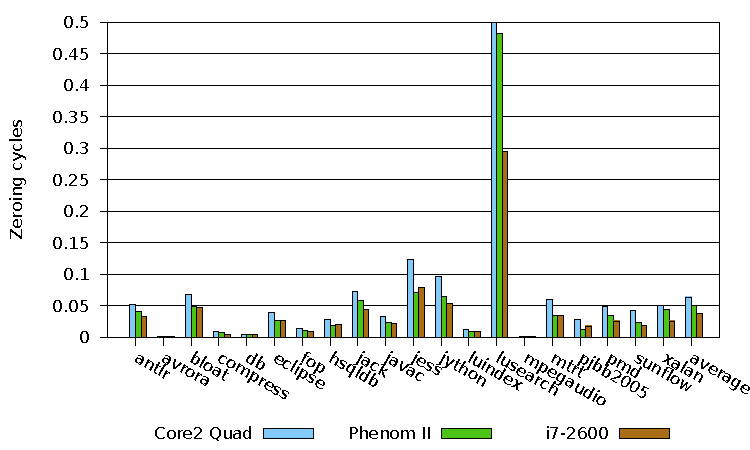
\includegraphics[width=\columnwidth]{figs/zerocost_intel.pdf}}
%  \subfigure[BytesZeroed / BytesBurstTransactionsTransferred\label{fig:zerobus}]{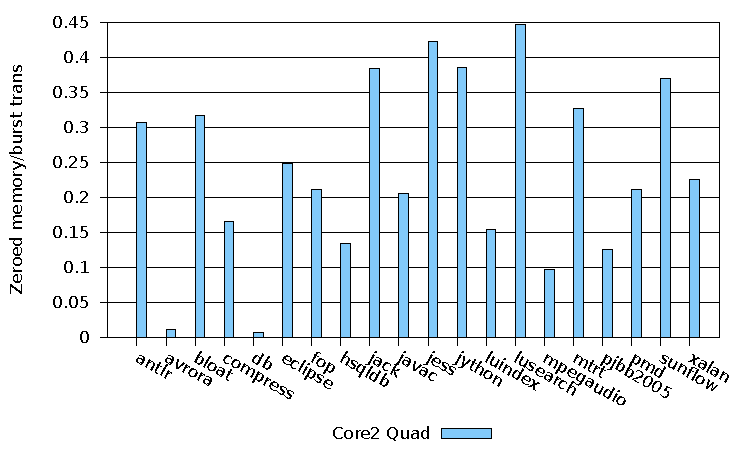
\includegraphics[width=1.0\columnwidth]{figs/zerobus_core.pdf}}
%  \caption{The cost of zero initialization}
%\end{figure*}

